\chapter{序論}
\label{chap:introduction}

\section{背景}
\label{section:background}

コンピュータの管理者は,動作中,あるいはカーネルパニックなどによって停止したコンピュータの情報を監視・解析することが必要となる場面がある.
動作中のコンピュータ自身に対しては,同一ホスト内のtopコマンドやpsコマンドを用いて,プロセスの一覧を得たり,gdbコマンドを用いてプロセスをトレースし,プロセスの状態を把握する.
ユーザー空間ではなくカーネルのデバッグしたい場合は,kdbと呼ばれるデバッガを,カーネルビルド時に有効にすることで,使用することができる.

論理的に停止したコンピュータに対しては,kdumpと呼ばれる機構を通してメモリダンプを静的に解析し,原因の究明をする.
また,状態を監視したいホストを物理的なマシンではなく,仮想マシンとして起動し,qemuやXenなどの基盤上でlibvmiなどを通して状態を解析する手法がすでに存在している.

上述した状況は,コンピュータの管理者,すなわちroot権限を保持している人にとって可能な手法である.

一方で,データセンター管理者など,大量の物理サーバーを保持し,顧客に貸し出している人の場合,上記の手法を使用することはできない.
通常は,顧客の情報にアクセスすることはするべきではないが,例えば貸し出しているサーバーがマルウェアなどに感染するなどした場合に事業者としての責任として,原因究明や現状調査のために,
解析する必要が出てくる可能性がある.

サーバーを貸し出している会社は,本来はセキュリティ対策として,サーバーを稼働しているオペレーティングシステム上に,セキュリティソフトを入れたいが,大量にあるコンピュータの全てにセキュリティソフトを入れることは容易ではない.
当然,顧客からrootパスワードを知らされることもないため,ログインをすることもできない.

\begin{figure}[htbp]
    \caption{libvmiを用いる際のアーキテクチャ}
    \label{fig:zentai}
    \begin{center}
        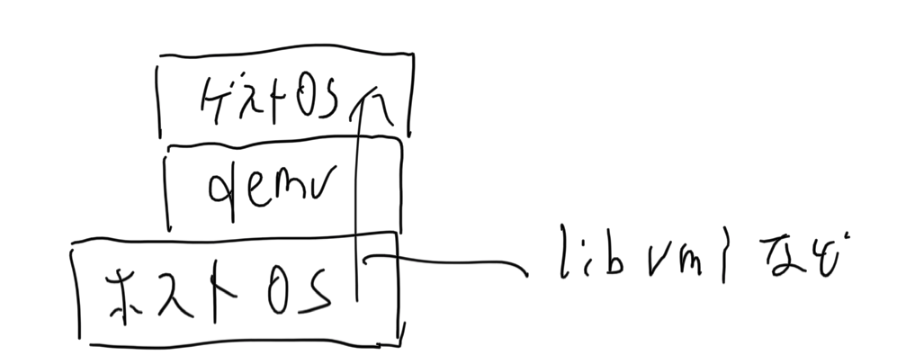
\includegraphics[bb=0 0 1000 340,width=15cm]{img/tegaki/01_vm.png}
    \end{center}
\end{figure}

\section{課題}
\label{section:problem}

\ref{section:background}で述べたように,データセンターの管理者は,顧客に貸し出している物理的なコンピュータの内部の状態を知ることはできない.
すなわち,死活監視として,ネットワーク越しの監視を行うことは可能であるが,コンピュータのオペレーティングシステムにおけるコンテキストを知ることはできない.
オペレーティングシステムの内部で起こっていることは,当然,通常は知るべきではないが,マルウェアに感染した場合,意図しない挙動を起こした場合,あるいはカーネルパニックに陥った場合,
これらの状態の時に,どの状態でも監視・解析を行うことができるツールが存在しない.

VMを用いた解析では,様々な解析手段がすでに豊富にあることは,\ref{section:background}で述べ,後述するとおり,VMを管理している物理的なコンピュータに以上が起きた場合に対処ができない.

大量の物理的なコンピュータに対する監視の場合,ネットワーク越しの死活監視,あるいはコンピュータの中でプロセスとしてセキュリティソフト,あるいは状態監視ツールを起動するほかない.
この手法は,大量のコンピュータに適用するのは,現実的ではない.
第一に顧客に貸し出すサーバーのリソースを微量でも使用してしまうという点.
第二に,全てのサーバーにセットアップするのが大変だという点(加筆が必要)

また,このプロセスとして起動する方法は,物理的なコンピュータのオペレーティングシステムがカーネルパニックに陥った際,コアダンプの解析を行う他に解析手段が存在しない.
コアダンプの設定を正しく行っていれば,静的ファイルを解析することは可能であるが,ストレージの不足など,不足の事態によって,ダンプを取ることができない可能性も存在する.

さらに,マルウェアなどに感染し,ログインをして解析することが危険にさらされる可能性もある場合,コンピュータにログインすることが推奨されない場合も存在する.

以上のことをまとめて,本研究における解決したい課題として,ネットワーク越しにある物理的なコンピュータに対して,電源さえ入っていればリアルタイムで安全に解析可能なオペレーティングシステムの監視・解析ツールが存在しないこと,と定義する.

% 背景で述べたRDMA NICを用いた解析手法では,メモリの物理アドレスを指定し,逐次的に値を取得し外部から復元していくが,

% これはここに書くべきではない.
% 書くべきは,VMなどの問題点.

\section{目的}
\label{section:purpose}

本研究では,大規模データセンターのような,大量かつ様々な環境の物理的なコンピュータを管理する現場において,
root権限がない中でネットワーク越しにあるコンピュータの状態を一元的に把握できることを示すことで,\ref{section:problem}で述べた問題を解決することを目指す.

この章で述べた様々な環境とは,同じバージョンのオペレーティングシステムでもビルドする際の設定によって,挙動が変わるという意味である.

本研究の実装によって,事前に与える情報が少ない中で,オペレーティングシステムのコンテキストを復元できることを示すために,
タスクキューに乗っているプロセスの一覧を取得することを目指す.

% そこで本研究の目的として,問題の章であげた3つの情報,Linuxカーネルのバージョン,System.mapの情報およびカーネルコンフィグのうち,
% System.mapおよびカーネルコンフィグの情報をRDMA NICを用いて復元する.
% また,Linuxカーネルのバージョンを知ることさえできれば,どのようなカーネルコンフィグを持つコンピュータに対しても,
% RDMA NICを通してプロセスリストの一覧を取得できることを実証する.

% この目的を達成するため,本研究では,いくつかの段階に分けてネットワーク越しにあるコンピュータに対して監視・解析を行っていく.
% 第一の工程として,RDMA NICを用いて,監視対象ホストのメモリを全探索し,
% メモリに落ちているSystem.mapのうち,\verb|init_task|が配置されている仮想アドレス空間に関する情報と,
% Linuxカーネルにおける\verb|__phys_addr|関数,\verb|task_struct|型を決定するためのカーネルコンフィグに関する情報を収集する.

% 次の工程として,収集したカーネルコンフィグを元に手元のコンピュータでLinuxカーネルのソースコードに対してプリプロセスの処理を行い,task_struct型を確定する.
% さらに,ソースコード上にある\verb|__phys_addr|関数の実体を収集する.

% 最後に,この工程で得られた情報をもとに,libtlpで提唱されている手法を用いて,プロセスの一覧を正しく取得できることを確認する.

\section{本論文の構成}

\ref{chap:related_works}章では、既存の解析基盤や様々な解析手法と,基盤技術として使用することになるRDMAの既存の実装について述べる.

\ref{chap:approach}章では、本研究のアプローチとして,メモリからオペレーティングシステムのコンテキストの復元に必要な情報について述べる.

\ref{chap:implementation}章では、本研究で実装したものについて述べる(加筆)

\ref{chap:evaluation}章では、本研究における評価として,Linuxカーネルのバージョンのみが与えられた状態でプロセスリストの一覧を取得できることを示す.

\ref{chap:conclusion}章では、本研究に関する結論と,今後の課題について述べる.
